\chapter{Solution Design}
\label{sec:solution}

\section{Business Process Model and Notation}
Business Process Model and Notation (BPMN) is a notation developed by the Object Management Group (OMG) whose purpose is to address the gap between the design and implementation of business models. BPMN aims to provide a standardized notation for all business users to facilitate the drafting, implementation, and monitoring of the business process and enhance the collaboration between all involved parties \cite{BPMN_tech_report}. Several phases of the BPMN lifecycle are discussed in \cite{BPMN_fundamentals}: Process Discovery, Process Identification, Process Modeling, Process Analysis, and Process Redesign.

\begin{figure}[h]
    \centering
    \caption{An example of BPMN diagram}
    \includegraphics[width=1.0\textwidth]{tum-resources/images/example_process.png}
    \floatfoot{generated using https://www.signavio.com based on \cite{diagram_source_01}}
\end{figure}

BPMN offers a variety of Elements to choose from to guarantee a comprehensive use case \cite{BPMN_tech_report}. The five basic elements categories are:

\begin{enumerate}
    \item Flow Objects
    \item Data
    \item Connecting Objects
    \item Swimlanes
    \item Artifacts
\end{enumerate}

The Flow Objects are a business process's primary components, consisting of Events, Activities, and Gateways. In this work, the \textbf{start event} and the \textbf{end event} are used. As their names suggest, the start and end event indicates that some specific process or choreography will start or end. BPMN offers many types of activity for different uses. However, this work will only focus on the basic activity (\textbf{Task}) for simplicity. A task is an atomic activity, which indicates work performed by companies within a process and is used when the work cannot be torn down into a finer detail level. The work focused on two types of gateways: \textbf{Exclusive} and \textbf{Parallel Gateways}. The Exclusive Gateways are used to diverge alternative possibilities within a process flow. Based on the conditions that occurred, only one path can be chosen. On the contrary, Parallel Gateways are used to create parallel paths considering no conditions, which indicates that two tasks can happen in the meantime. 

Data refers to the data objects used to indicate what kind of data a task would require as input or generate as output. Connecting objects include the different kinds of flows from one activity to another. The work majorly focused on \textbf{sequence flow} which is used to show the sequence of how the activity is going to be executed. The graphic elements are grouped using swimlanes by putting all the relevant elements inside one swimlane. There are two types of swimlanes: pools and lanes. A pool represents a business participant in the business model, while a lane is the sub-partition within a pool. For example, a pool could be "the sales department" and it can contain two lanes, "employees of the department" and "the head of the department". Finally, the modeler can use artifacts to provide extra information about the business process. If needed, as many artifacts can be used as necessary.

Although a significant amount of BPMN elements are offered for use, this work only focuses on several certain types of elements in order to focus on developing the algorithms that automatically extract the business process elements. However, the algorithms offered by the work are intuitive and can be easily adapted to further use cases.

\section{Solution Strategy}
The input format taken for this work is considered pure text (\textit{.txt}) because this is the most common text format known to all business process participants and is free of additional styling information, which could cause possible inefficiency when extracting the information. The most crucial step before applying the rule-based information extraction algorithms is the tokenization and the part-of-speech (POS) tagging on the input textual description. Tokenization is a technique that divides texts into single words, i.e., tokens. Then, the tokens are annotated with the proper grammatical and syntactical information using part-of-speech tagging \cite{literature_review_2}. These two techniques are fundamental in the context of automatic information retrieval, for \cite{literature_review_1} suggests that many works in this research field have leveraged tokenization and POS tagging.

\begin{figure}[h]
    \centering
    \caption{Overview of pre-processing}
    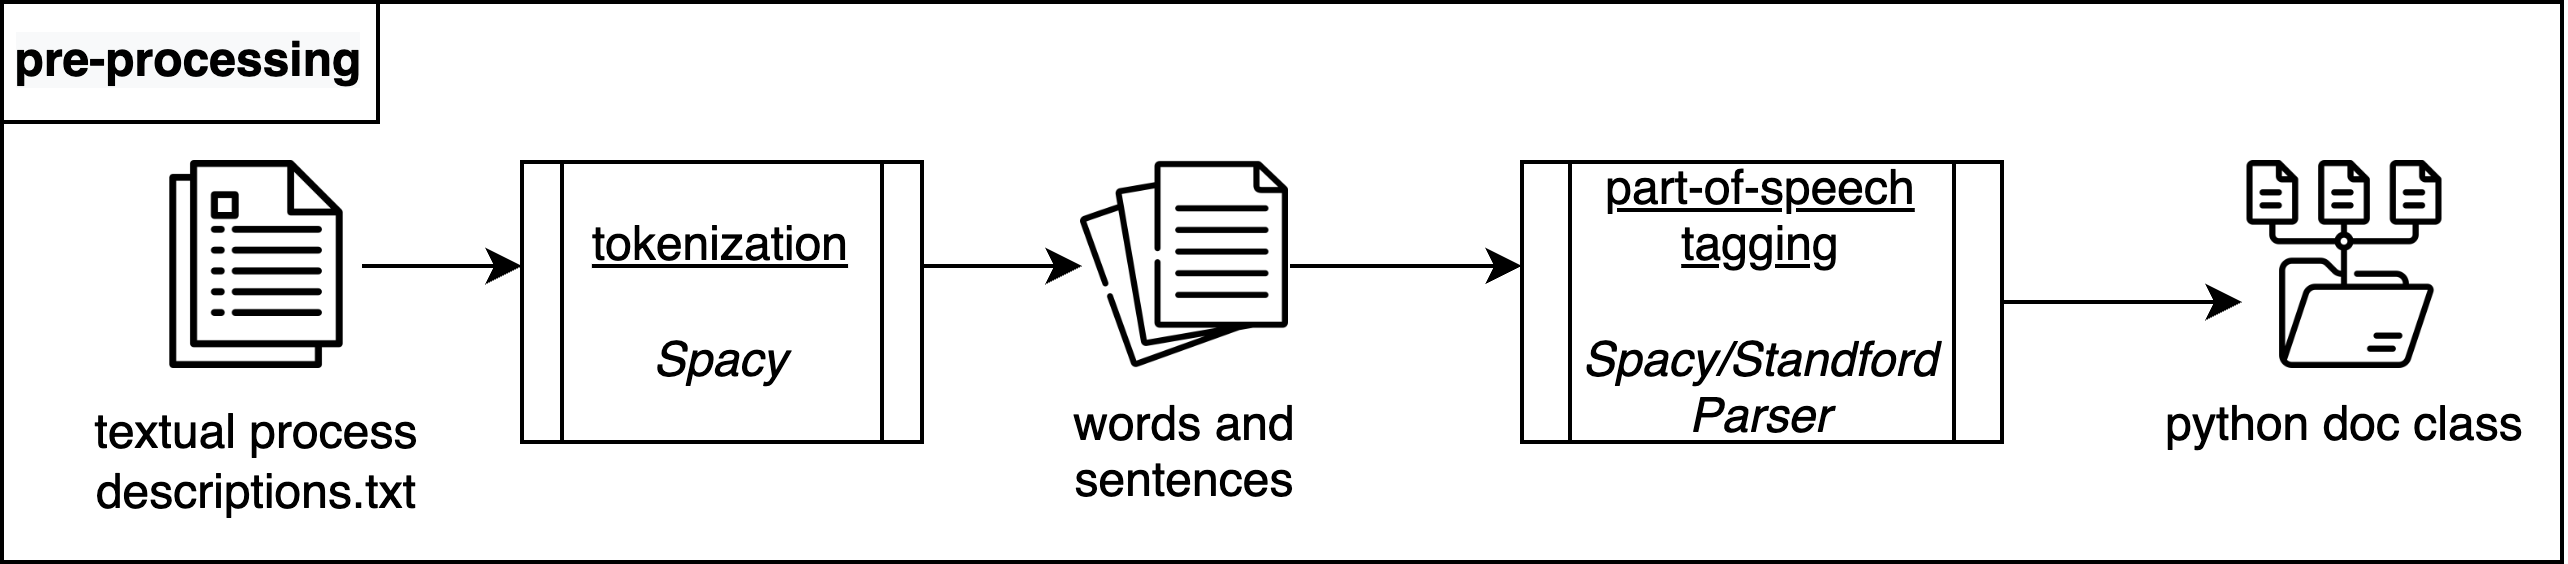
\includegraphics[width=0.8\textwidth]{tum-resources/images/theoretical_extraction_pre.png}
\end{figure}

Extracting information from documents written in text is not a simple task due to the nature of the complexity of natural language. Our approach will consider using textual process descriptions as input files in the format of \textit{.txt}. In the first step, the input file will be pre-processed. The documents will be split into sentences and words using tokenization. Then, the words in the sentence should be tagged with a proper grammatical label using the part-of-speech technique so that the relationship between words can be analyzed. An essential step of this part is to identify the business activities. \cite{t2m_5} and \cite{complement_1} suggest that the identification can be achieved by the pre-defined rules based on the grammatical properties of the words. Once the business activities are identified, they can be used as the fundament of the work.

\begin{figure}[h]
    \centering
    \caption{Two approaches to perform process extraction}
    \includegraphics[width=0.8\textwidth]{tum-resources/images/transformation_process.png}
\end{figure}

\cite{literature_review_5} suggests two categories of methods to perform process extraction exist. The first algorithm category uses a single mapping function $f$ to transform the textual descriptions into BPMN diagrams. Such mapping function $f$ is considered adequate by taking care of all available information in the context to help with solving problems. Nevertheless, $f$ could lead to low accuracy when the solutions need to be generalized or the input context differs. The second category of algorithms, which is adopted by this work, use a two-step function with an intermediate storage to perform the process model transformation. In the second approach, the transformation function $f$ is considered as a compound function consisting of two individual functions $ f_a $ and $ f_b $. Two functions have their roles, $ f_a $ is responsible for extracting the process-relevant information from the textual description and then storing the extracted information in data storage. $ f_b $ then access the information stored in the data storage, perform further analysis, and in the end, generate a BPMN diagram.

\section{Categorization of Issues}
\cite{t2m_1} identified four category of obstacles to performing the information extraction from natural language: \textit{Syntactic Leeway} describes the problem of inconsistency between the semantic and syntactic aspects of the textual representation. \textit{Atomicity} refers to the problem of adequately mapping the phase-activities. \textit{Relevance} checks whether some part of the text input is irrelevant to the process model, such as examples offered by authors, which helps the human reader to understand the described process but introduces noise for information extraction. \textit{Referencing} deals with the question of how to identify the references between sentences, e.g., the pronouns "This" and "it", from the sentence "After this step, it will be delivered to ...".

    \begin{table}[]
        \begin{center}
        \caption{\centering Obstacles in performing BPMN extraction}
        \label{table:obstacles}
        \begin{tabular}{ll}
        \textbf{Issue}\hspace{60mm} \\
        \hline
        1. Syntactic Leeway                                            \\
        \quad 1.1 Active/Passive Voice recognition                     \\
        \quad 1.2 Condition Recognition                                \\
        \quad 1.3 Missing Actor                                       \\
        \hline
        2. Atomicity                                                   \\
        \quad 2.1 Sentences Decomposition                              \\
        \quad 2.2 Subordinate Clauses                                  \\
        \hline
        3. Relevance                                                   \\
        \quad 3.1 Example Sentences and Explaination                   \\
        \quad 3.2 Meta Information                                    \\
        \hline
        4. Referencing                                                \\
        \quad 4.1 Anaphora                                            \\
        \end{tabular}
        \end{center}
        \floatfoot{Identified issues based on the work of \cite{t2m_1}}
    \end{table}

Within these four categories of obstacles, the work explored the potential problems more deeply. According to the nature of the issues identified, they are categorized into the four major challenges as listed in table \ref{table:obstacles}. 

\subsection{Syntactic Leeway}
\label{sec:solution:syn_lee}
Within the category \textit{Syntactic Leeway}, a major challenge to be overcome is the recognition of active and passive voice. A sentence with the same meaning can be expressed through two possibilities, namely, active or passive. Consider the following example: the first sentence is written in active voice, and the second in passive voice. 

\begin{itemize}
    \item A customer brings in a defective computer
    \item A defective computer is brought in by a customer
\end{itemize}


In the given example, two expressions here have the same semantic meaning; the two sentences' syntactic structures are totally different. In order to further illustrate the problem, the work used the \textit{displacy}, a visualization tool offered by \textit{spacy}, to visualize the syntactical relationship of the word components.

\begin{figure}[h]
    \centering
    \caption{syntactical visualization of the first example}
    \includegraphics[width=0.8\textwidth]{tum-resources/images/active_example.png}
\end{figure}

\begin{figure}[h]
    \centering
    \caption{syntactical visualization of the second example}
    \includegraphics[width=0.8\textwidth]{tum-resources/images/passive_example.png}
\end{figure}

In the active voice sentence, the actor of the sentence is indicated through the \textit{spacy dependency} \textbf{nsubj} and the actor in the passive sentence is indicated through \textbf{pobj}. Therefor, if the work wishes to extracted the correct actors in the process descriptions, this problem must be solved and the proper pre-processing must be performed so that the different extraction rules and be applied accordingly.  

Another issue to be addressed in this challenge category is recognizing conditional markers. Conditional markers are used to identify whether a sentence or a sub-sentence expresses a condition's meaning. There are majorly two group categories of conditional markers: 

\begin{enumerate}
    \item if
    \item else
\end{enumerate}

These two marker groups correspond highly to the if-else condition in the computer programming language. The if condition indicates what actions will happen after some specific condition, whereas the else condition indicates what will happen otherwise. The condition marker can also be expressed in various ways in natural language. Therefore it is challenging to correctly identify the conditional markers stated differently. 

\begin{itemize}
    \item If an error is detected, a repair activity is executed
    \item In case an error is detected, a repair activity is executed
    \item In case of an error, a repair activity is executed
\end{itemize}

From the examples above, it is not hard to find out that the conditions here express the same meaning yet are written with different styles. Therefore, it is not sufficient only to perform a single string matching activity because this will lead to the potential ignorance of some markers. Considering the mentioned properties of conditional markers, the work intended to use a multi-step recognition with the spacy dependency recognition and spacy matcher to ensure we have covered the broadest range of the conditional marker. 

Another challenge is the situation where sometimes the actor that is to be included in the lanes in the BPMN models are not explicitly expressed. This can happen due to several reasons, the first possible scenario is that the action is embedded in a subordinate sentence, and therefore there is no need for the main sentence to explicitly indicate who performs the action.

\begin{itemize}
    \item the room-service manager gives an order to the sommelier to fetch wine from the cellar.
\end{itemize}

In this sentence, the action "fetch wine from the cellar" should be performed by the "sommelier", yet purely extracting the action will lead to the Actor missing problem because this action is an \textit{object of a preposition (pobj)} from the preposition "to" \cite{dependencies_manual}. Therefore, it is sometimes necessary to perform a backwards-checking to see whether an actor is included in the main clause. 

Another possibility for the problem is using a passive voice sentence. Because in passive voices, the actor of the sentence is typically addressed using "by", yet this is not mandatory. Such component is also a \textit{agent dependency}, which represents the actor introduced by the preposition "by" who does the action \cite{dependencies_manual}. As a result of this phenomenon, when parsing a passive voice sentence that does not have an \textit{agent dependency}, it is not possible to find a valid actor, and therefore, we cannot place the action into the lanes correctly.

Finally, the last situation occurs when the direct actor of a action is not in the valid lane actor candidates. It is neither efficient nor wise to gather all actors in each sentence in textual descriptions and add use this actor list to construct the lanes. Only some actors that are relevant to the process descriptions are desired, the actor selection process problem will be further discussed in the Implementation section \ref{sec:implementation}.

\begin{itemize}
    \item CRS checks the defect and hands out a repair cost calculation back. The ongoing repair consists of two activities. The first activity is to check and repair the hardware
\end{itemize}

In the last sentence from the example above, the direct actor of the action is "The first activity". However, it is not appropriate to have "The first activity" listed in the lanes of the BPMN diagram. Although this action is carried out by the actor "The first activity", it is implicitly indicated that the real actor performing this task is the "CRS". To address the latter challenges, the work propose the idea to find the real actor in the context if the current actor is not listed in the real actor list. Further technical details will also be explained in the Implementation section \ref{sec:implementation}.



\subsection{Atomicity}

In the next step, we would like to discuss the \textit{atomical} challenges introduced by the complexity of the sentences. \textit{Spacy} has the ability to identify and separate the sentences in a document input. The segregated sentences can then be used for information extraction, which works well with simple sentences. However, if the sentence is complicated and is consisted of several parts or clauses, information extraction becomes very difficult. \footnote{https://spacy.io/api/doc\#sents}

\begin{enumerate}
    \item A small company manufactures customized bicycles.
    \item A customer brings in a defective computer and the CRS checks the defect and hands out a repair cost calculation back.
\end{enumerate}

The first sentence is a typical simple sentence structured with subject–verb–object word order. In this case, the extraction strategy is straightforward: Once the location of the verb is located, the subject and the object of the sentence can be traced very easily using the \textit{spacy dependencies}. The token "company" has the \textbf{nsubj} dependency, and the token "bicycles" has the \textbf{dobj} dependency to the verb "manufactures". "nsubj" represents the nominal subject and serves as the syntactic subject of a clause, whereas the "dobj" stands for direct object indicating it is the accusative object of the verb \cite{dependencies_manual}.

However, the second sentence is more complex than the first, for it comprises several clauses connected through Coordinating conjunctions, namely "and". Dealing with such sentences without further operations could be very challenging. A single extraction strategy could be insufficient, and essential information could be missed. Therefore, illustrated by \cite{t2m_1}, the work develops a new sentence pre-processing technique based on the divide and conquer principle. To achieve this, the \textit{The Penn Treebank} is leveraged to perform constituency parsing. POS tagging only assigns the tokens with part of speech labels, which contributes little to the sentence decomposition. Thus this work uses constituency parsing to perform the full syntactic analysis of the input textual descriptions by generating phrase-structure trees \cite{parser_01}. As illustrated in figure \ref{img:con_par}, a sentence can be parsed into a tree structure through constituency parsing, and the correspondent full syntactic tags are added to each token \cite{penn_tree_explanation_1} \cite{penn_tree}. Once the sentence is constituency parsed, we are able to analyze the complex sentences and, based on the syntactic tags, divide a complex sentence into several simple sentences where only one verb is contained in a clause. This proposed approach will ease the burden of performing information extraction and delivers a more accurate result.

\begin{figure}[h]
    \centering
    \caption{a constituency parsing example}
    \label{img:con_par}
    \includegraphics[width=0.8\textwidth]{tum-resources/images/Constituency_Parse.png}
    \floatfoot{generated using https://corenlp.run/}
\end{figure}
 

\subsection{Relevance}
\label{sec:solution:relevance}
Another obstacle in automated information extraction is the relevance of the sentences to the whole process. The examples offered in the textual descriptions used to generate BPMN diagrams assist the human reader and modeler in understanding the business process more concretely. However, such examples and explanations can cause confusion when using the algorithm to extract business processes because the algorithms can only perform a restricted semantic analysis and therefore is often difficult for machines to decide which information is relevant to the business process and which is an example or explanation. 

The work of \cite{pet_dataset} developed a gold-standard corpora, PET dataset, for the researchers to perform evaluations on their work with BPMN, the source from the PET dataset is from the source used in \cite{t2m_1}, on which this work is built on. The PET dataset can also help to address the problem of irrelevant information, for all the relevant information is marked within the dataset. 

\begin{itemize}
    \item While the kitchen and the sommelier are doing their tasks, the waiter readies a cart \textbf{(i.e., puts a tablecloth on the cart and gathers silverware)}.
    \item Otherwise, the matter details \textbf{(types of action)} are captured and provided to the Cashier.
    \item However, if inconsistencies exist, \textbf{e.g. because the ordered product is not of the expected quantity or quality}, the cost center manager rejects the AP.
\end{itemize}

We offer some examples here to better illustrate the meaning of the information about the examples and explanations. In the first two examples, we can see that the explanation information is given to illustrate what the phrases "readies a cart" and "matter details" mean. In the third given example, an example is offered to explain what the "inconsistencies exist" specifically indicate. This sort of information can be essential for the reader and modeler to understand the context of the specific phrase and terminology because some words are highly domain-specific and, thus without the explanations offered by the domain expert hard to understand. 

\begin{itemize}
    \item \textbf{A small company manufactures customized bicycles.} Whenever the sales department receives an order, a new process instance is created.
    \item \textbf{The Evanstonian is an upscale independent hotel.} When a guest calls room service at The Evanstonian, the room-service manager takes down the order.
\end{itemize}

In the given examples, the black-marked sentence is considered as process irrelevant information according to the PET dataset. Although such sentences offered some helpful information about the whole process, in the former case, through the sentence, we can learn about the functionality of the small company, which is about customized bicycle manufacturing, and in the latter case, we learned that the Evanstonian is the name of a hotel. However, This information is not directly relevant to the business process; even without them, the modeled diagrams are still considered complete. Therefore, such information can be considered as meta-information about the process.

Such process irrelevant information, on the one hand, increases the understandability of the textual description for human interaction but, on the other hand, also increases the difficulty when processing the sentence using computer algorithms. Therefore, the work tried to filter the irrelevant information firstly by performing the semantic analysis on verbs and examining a word stop list and then using the Large Language Model to perform a more thorough semantic analysis. 

\subsection{Referencing}
\label{sec:solution:referencing}
The last group of challenges is the referencing problem, namely the problem concerning the anaphora resolution. Anaphora is the phenomenon that the actual words are replaced through a pronoun. This can happen in several places, within a complicated clause, a subordinate clause, or another clause. Consider the following examples:

\begin{itemize}
    \item If the \textit{customer} decides that the costs are acceptable, the process continues, otherwise \textbf{she} takes her computer home unrepaired.
    \item The storehouse checks the required quantity of each part. If the \textit{part} is available in-house, \textbf{it} is reserved. If \textbf{it} is not available, \textbf{it} is back-ordered.
    \item Asking the customer \textit{whether he is generally interested} is also important. If \textbf{this} is not the case, we leave him alone.
\end{itemize}

The black-marked tokens are the so-called anaphora, i.e., they are pronouns used to refer to the actual words previously used (marked using italics) in the same discourse. These examples show that the anaphora phenomenon can occur not only once but multiple times, as suggested in the second example. Furthermore, anaphora can refer to a word mentioned previously but can also refer to an action, as the third example indicated. The pronoun "this" in the context no longer refers to a single word but to the action "whether he (the customer) is generally interested". Therefore, performing an anaphora resolution is vital so that the extracted information to be used later for process model generation is accurate. 

\section{Solution Approach}
As stated in the previous sections, extracting information from textual descriptions is a complex task but still needs to be solved. The work \cite{t2m_1}, considered as state of the art, also suggests that the work aims not to replace the human modelers but to assist them to save time and make the work easier for them. This work aims to reproduce the work of \cite{t2m_1} with more advanced technologies and make appropriate improvements. Therefore, some deviations in the work from output can be accepted. However, an easy-to-use interface is desired because our system's user group is aimed at the participants in the business process who have little technical knowledge. 

Nevertheless, we have to find suitable tools and algorithms to address the problem listed in table \ref{table:obstacles}, to achieve a result as accurate as possible. As a result, syntactic and semantic analysis should be performed upon the input textual descriptions, therefore, the work exploits the opportunity to find the appropriate tools to facilitate the information extraction procedure. After thorough research, we will use Spacy, which is reported to have a high accuracy \cite{complement_1}, as our primary tool for natural language processing to perform tokenization, POS tagging, as well as the fundamental natural language process tasks, furthermore, WordNet, a constituency parser and an anaphora resolver are chosen as complements. The tools will be used in a different stage of information determination and extraction, guaranteeing that the system is designed with low coupling and adapted to further individual use. The intermediate data is stored in Python class, which allows the program to access and store the data with low latency.

\begin{figure}[h]
    \centering
    \caption{class diagram}
    \label{class_diagram}
    \includegraphics[width=0.8\textwidth]{tum-resources/images/uml.png}
\end{figure}

In order to store the data more efficiently, the work also creates several Python classes representing the different abstraction levels to store the extracted information. After the textual description is analyzed as a whole, it is a good idea to store each sentence in a data structure. The class \textit{SentenceContainer} is used for the storage of the separated sentence. In \textit{spacy}, the divided sentence is called a \textit{span} object, with which the work is able to perform further complex operations. A sentence stored in \textit{SentenceContainer} can then be divided into several parts (\textit{Process}) according to syntactic tags using the constituency parsing to ensure that each part only contains only one verb, which makes the information extraction follows the divide-and-conquer principle. \textit{Process} consists of three essential components: \textit{Actor}, \textit{Action}, and \textit{Resource}. The subject of a clause is stored in the \textit{Actor}, whereas the \textit{Resource} stores the object. \textit{Action} stores the verb as well as the conjunctions of that verb. \textit{Activity}, \textit{ConditionalBlock} and \textit{AndBlock} are used to build the BPMN flow. As the names suggest, \textit{Activity} represents a single BPMN Task, \textit{Activity} and \textit{ConditionalBlock} represent branches inside the Exclusive and Parallel Gateways.

This work also intends to leverage the power of the \textit{in-context learning} approach to perform the correction on the generated BPMN diagram. Large Language Models such as \textit{GPT} from OpenAI and \textit{Bard} from Google are pre-trained using huge amounts of data by leveraging the advancement of deep learning. The problem-solving in the NLP field begins to shift from designing specific solution architectures to using pre-trained Models \cite{LLM_2}. \cite{LLM_1} reveals the possibility to perform a question-and-answer dialog to extract knowledge using in-context learning using \textit{GPT-3} for the first time. Based on the prompt suggestions given by \cite{LLM_1}, this works uses the \textit{GPT-4} to correct and refine the output generated using the rule-based information extraction. Four major tasks are given to the \textit{GPT-4}: 

\begin{enumerate}
    \item Irrelevant information recognition and removal
    \item Expressions refinement
    \item Anaphora resolution enhancement
    \item Gateways checking and adjustments
\end{enumerate}

For each Task, a detailed task description and two examples will be provided first to have the LLM learn the desired output. 













